Maintenant que vous avez bien compris le fonctionnement d'un moteur DC et du pont H qui permet de le contrôler, il est temps de passer à la pratique! Durant ce premier hands-on, vous allez pouvoir connecter votre premier moteur DC ainsi que de le contrôler à l'aide des signaux électriques.\\

Dans la section précédente, vous avez pu vous familiariser avec le schéma d'un pont H. Ce circuit peut être réalisé soit à partir de composants discrets séparés, typiquement dans des applications nécessitant de hautes puissances et donc des composants plus conséquents, mais il existe également des versions intégrées dans des puces électroniques prêtes à l'emploi. Utilisées essentiellement dans des petites applications lorsque les courants et tensions ne sont pas trop élevés, celles-ci offrent un gain en taille et en coût qui permet de réaliser un petit circuit de contrôle assez facilement. C'est cette seconde approche que nous utiliserons dans ce projet, à l'aide du composant L293D de Texas Instruments.\\

Le L293D comprend 4 demi-ponts H, comme vous pouvez le voir à la Figure~\ref{L293}. Ces demi-ponts peuvent être utilisés soit séparément, soit par 2 pour former le pont H tel que vous l'avez vu dans la section précédente. Quelques petites observations intéressantes sur ce schéma:
\begin{itemize}
\item Un signal de contrôle supplémentaire (EN) permet de déconnecter la borne Y de son circuit de contrôle.
\item Le L293 nécessite 2 alimentations séparées: une pour le contrôle des interrupteurs et une pour alimenter le pont H (et donc le circuit connecté à sa sortie). Cette séparation est très pratique, par exemple pour contrôler des moteurs qui nécessitent une tension élevée (9V dans notre cas), à l'aide de signaux provenant d'un microcontrôleur (typiquement 5V). Dans ce premier hands-on, pour la simplicité, les 2 alimentations seront connectées à 5V.
\item La masse du circuit est connectée à 4 broches du boîtier. Cela permet non seulement d'assurer une bonne conductivité, mais aussi de dégager la chaleur générée par les forts courants qui peuvent apparaître dans la puce. Cette chaleur est alors redistribuée dans la breadboard ou le PCB.\\
\end{itemize}

\begin{figure}[!t]
\centering
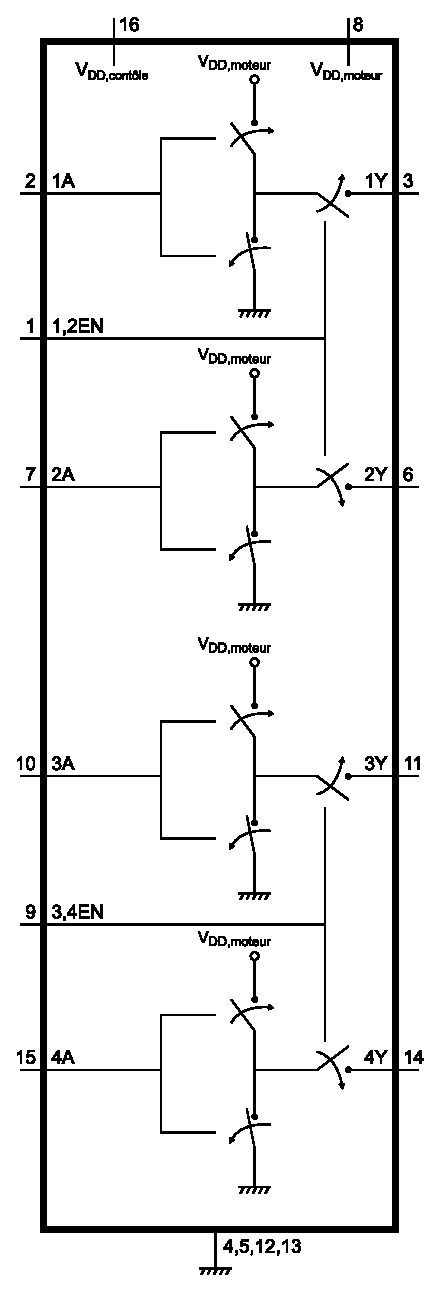
\includegraphics{L293.eps}
\caption{Schéma simplifié du L293D. Les numéros indiqués près des entrées/sorties correspondent aux numéros des broches de la puce.}
\label{L293}
\end{figure}


Vous pouvez maintenant réaliser sur une breadboard le petit circuit de contrôle illustré à la Figure~\ref{circuit}. Ce circuit utilise 2 demi-ponts H du L293. ATTENTION à ne pas oublier les diodes et à les connecter dans le bon sens. Comme expliqué précédemment, si ces diodes ne sont pas connectées correctement, le courant qui apparait lors de la décharge de l'énergie magnétique risquerait d'endommager le L293. N'hésitez pas à demander à l'un des membres du Club Elec de vérifier votre circuit si vous avez le moindre doute!\\

\begin{figure}[!t]
\centering
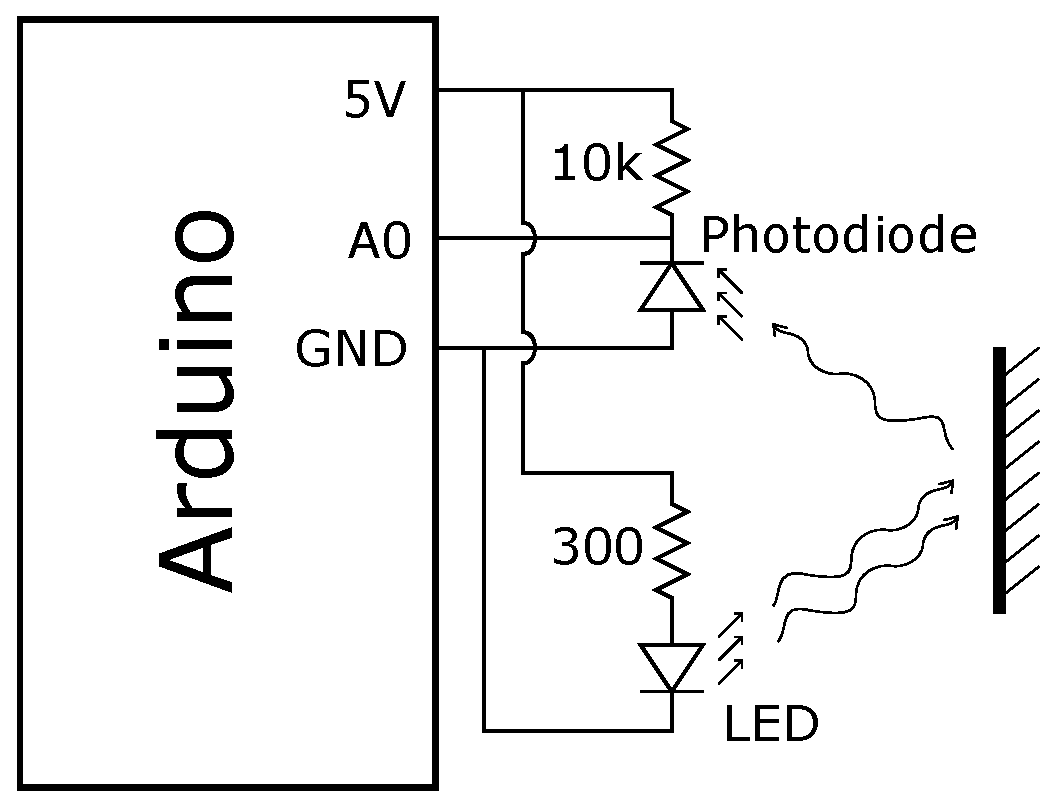
\includegraphics{circuit.eps}
\caption{Contrôle d'un moteur à l'aide du L293D. Les broches non indiquées sur le schéma peuvent être laissées flottantes ou connectées à la masse.}
\label{circuit}
\end{figure}

Essayez maintenant de connecter les signaux de contrôle (EN, A1, A2) à l'alimentation de 5V ou à la masse. Qu'observez-vous sur le moteur? Cela correspond-t-il bien à ce à quoi vous vous attendiez? Vérifiez avec le comportement attendu repris dans la Table~\ref{signal}.\\

\begin{table}[!t]
\caption{Signaux de contrôle pour le moteur DC}
\begin{center}
\begin{tabular}{|l|l|l|l|}
\hline
\textbf{EN}& \textbf{A1} & \textbf{A2} &\textbf{Moteur}\\
\hline
5V & 0V & 5V & Tourne dans un sens\\
5V & 5V & 0V & Tourne dans l'autre sens\\
5V & 0V & 0V & Freine\\
5V & 5V & 5V & Freine\\
0V & X & X & Libre\\
\hline
\end{tabular}
\label{signal}
\end{center}
\end{table}

S'il vous reste du temps, connectez l'entrée EN à un générateur de signal et générez un signal rectangulaire entre 0 et 5V. Que se passe-t-il lorsque vous faites varier le duty-cycle (rapport du temps à 5V et à 0V) de ce signal.
